\documentclass{article}
\usepackage[T1]{fontenc}
\usepackage{lmodern}
\usepackage{graphicx}
\usepackage{amsmath,amssymb}
\usepackage[a4paper,margin=2cm]{geometry}
\usepackage[absolute,overlay]{textpos}
\setlength{\TPHorizModule}{1mm}
\setlength{\TPVertModule}{1mm}
\usepackage[indonesian]{babel}
\usepackage{hyperref}
\setlength{\emergencystretch}{2em}
% unit: Halaman 33

\begin{document}

% === Halaman 33 (python/native) ===

33

• Vigènere Cipher menggunakan 

tabel 

Vigènere 

– 

dinamakan 

Vigenere 

square, 

untuk 

melakukan enkripsi dan dekripsi. 

• Setiap 

baris 

i 

di 

dalam 

bujursangkar menyatakan huruf-

huruf cipherteks yang diperoleh 

menggunakan 

Caesar 

Cipher 

dengan kunci k = i.

• Artinya, setiap baris i merupakan 

pergeseran huruf alfabet sejauh i 

ke kanan

% deskripsi: gambar native xref 145
\noindent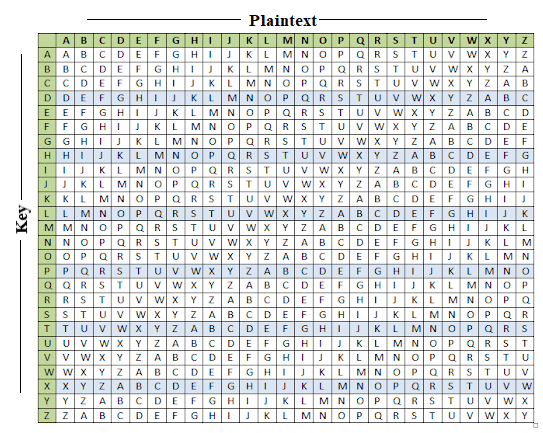
\includegraphics[width=0.85\textwidth]{../../images/python/page_033_img_01.png}

\end{document}
